\subsection{Hardware/Software mapping}
\paragraph{Systems}\mbox{}\\
This program is inherently a documentation tool which map research articles goals and conclusions in a searchable context. This requires the program to be stable and reliable, especially  in the context of data preservation. \\The program is split into two components, a client, and an external database  server. The user will run a client on his computer which will communicate with the server which runs the application logic and storage. The user client will feature data preservation, to enable offline functionality, but only to a limited, extend. This report primarily focuses on the server, if any questions to the user client should occur,  please refer to the according Blue SDD.\\ \\
All user clients will contact a single server. To solve this, the server will be multithreaded, which allows for multiple users interacting with the server at the same time, but  At the current scope of the program, this is possible due to a low amount of users, but should this system expand a new design should be conceived. \\
\begin{figure}[H]
	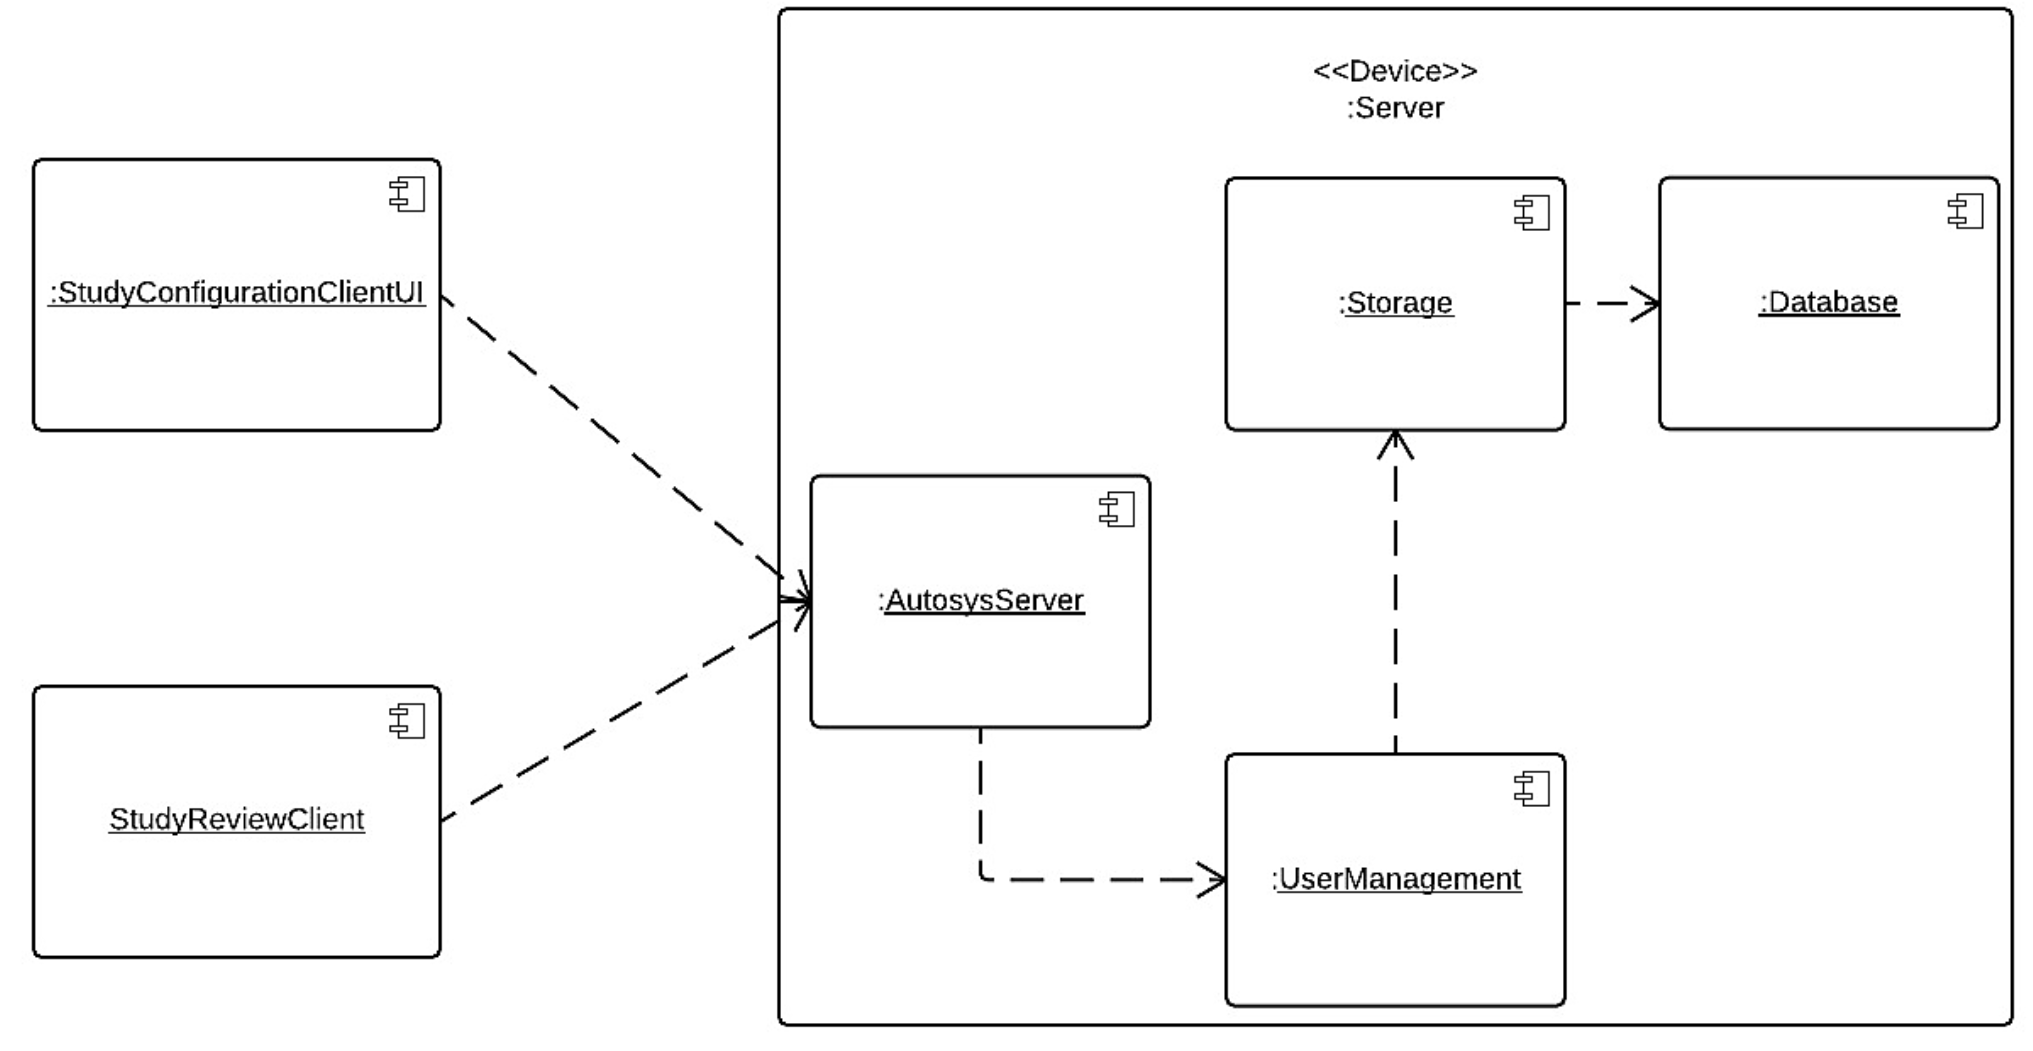
\includegraphics[width=\textwidth]{mappingImage}
	\caption{ Software mapping of prior subsystem decomposition. Note that the components UserManagement, PaperManagement, and StudyManagement has been collapsed into a single unit called UserManagement }
\end{figure}
\paragraph{Program components}\mbox{}\\
The server will be implemented in C \# as requested by the client. By using C \#, we can utilize Microsoft expansive database systems and interfaces especially in regards to the database. Additionally, this also makes the program easier to maintain, since C \# is a well-known language and utilizes the .NET framework. As communication between the server and the clients, we plan to communicate with HTTPS  request containing JSON object. This will make it easier to implement future changes and even completely replace the client's user interface with a more modern solution like a web page
\\\\
To achieve fast database responses, we will implement an entity framework database, which utilizes Microsoft's .NET framework to optimize database queries. It is assumed that this takes advantage of optimized queries and features implemented by Microsoft database experts. Furthermore, a future feature may be implemented to cache the result of large queries for quick access. This allows the server to respond hastily to large queries, which have previously been used. This will only be implemented for queries on data that is less likely to change. As a result, a memory trade-off may occur, which can be negated by using limits on how much memory and how many queries are cached. By way of example, the last x number of query results to the server could be cached for repeated use. The design goal is a refinement of the non-functional requirement "high performance" in the Requirement Analysis Document.